\section{A Readers and Writers Lock}

Different systems have different access requirements.  Threads should be
allowed to execute a particular part of the code, known as the \emph{critical
  section}, only under particular circumstances.  In this section we study a
classic access-control problem, the \emph{readers and writers problem}.

Consider a database, shared by a number of threads that carry out transactions
on the database.  We do not want different transactions to interfere with one
another.  Some threads simply read the database: we call these \emph{readers}.
It is fine to allow multiple readers to perform transactions concurrently:
they will not interfere with one another.  Some threads both read and write
the database: we call these \emph{writers}.  We should not allow two writers
to perform transactions concurrently; nor should we allow a reader and writer
concurrently.

We require an object to mediate access to the database, which we call a
\emph{readers and writers lock}.  We will take this
object to have the interface in Figure~\ref{fig:readers-writers}.  Each thread
should call the relevant operation before and after using the database.  For
example:
\begin{scala}
  ... // Operations not using the database.
  rw.readerEnter // Entry protocol.
  ...// Operations reading the database.
  rw.readerLeave // Exit protocol.
\end{scala}
%
The |readerEnter| and |writerEnter| operations should each block until it is
safe for the thread to use the database.

%%%%%

\begin{figure}
\begin{scala}
trait ReadersWritersLock{
  /** A reader enters the critical section. */
  def readerEnter(): Unit
  /** A reader exits the critical section. */
  def readerExit(): Unit
  /** A writer enters the critical section. */
  def writerEnter(): Unit
  /** A writer exits the critical section. */
  def writerExit(): Unit
}
\end{scala}
\caption{The interface for a readers and writers lock.}
\label{fig:readers-writers}
\end{figure}

%%%%%

We will see two implementations of the readers and writers lock.  The first,
in Figure~\ref{fig:readers-writers-monitor0}, is fairly simple.  It maintains
variables |readers| and |writers| that record the number of readers and
writers currently in the critical section.  It aims to maintain the invariant  
\[\mstyle
(\sm{readers} = 0 \lor \sm{writers = 0}) \land \sm{writers} \le 1.
\]
That is, there are not simultaneously readers and writers, and not more than
one writer. 

%%%%% 

\begin{figure}
\begin{scala}
class MonitorReadersWriters0 extends ReadersWritersLock{
  /** Number of readers currently in the critical region. */
  private var readers = 0

  /** Number of writers currently in the critical region. */
  private var writers = 0

  /* Invariant: £$(\sm{readers} = 0 \lor \sm{writers = 0}) \land \sm{writers} \le 1$£. */

  private val lock = new Lock

  private val cond = lock.newCondition

  def readerEnter() = lock.mutex{
    cond.await(writers == 0)
    readers += 1
  }

  def readerExit() = lock.mutex{
    assert(writers == 0); readers -= 1; cond.signalAll()
  }

  def writerEnter() = lock.mutex{
    cond.await(readers == 0 && writers == 0)
    writers += 1
  }

  def writerExit() = lock.mutex{
    assert(writers == 1 && readers == 0); writers -= 1; cond.signalAll()
  }
}
\end{scala}
\caption{A simple implementation of a readers and writers lock.}
\label{fig:readers-writers-monitor0}
\end{figure}

%%%%%

The implementation uses a single |Condition| for signalling.
Each of the entry operations waits until the relevant condition holds, and
records its own entry.  Each of the exit operations records its exit, and
signals to all waiting threads.

Consider the point at which a thread calls |writerExit|.  At this point, there
might be threads wanting in |readerEnter|, |writerEnter|, or both.  Without
additional state, there is no way for the exiting writer thread to know which
threads to signal to.  The only option, then, is to use |signalAll|.  If there
are both waiting readers and writers, it is nondeterministic which will
subsequently acquire the lock first.  If a writer goes first, it will enter
the critical section, setting $\sm{writers} = 1$, but all other readers and
writers will have to wait.  If a reader goes first, it will enter, setting
$\sm{readers} = 1$, all the other readers will subsequently enter, but the
writers will have to wait again.

\begin{instruction}
Make sure you understand the details of the implementation.
\end{instruction}

We can test the readers and writers lock using linearizability testing.  We
can run threads that repeatedly enter and exit, as either readers or writers.
We can then specify the lock as an abstract datatype whose state records the
current numbers of readers and writers, and that maintains the above
invariant.  Figure~\ref{fig:rw-seq-spec} gives a class~|SRW| of suitable
sequential specification objects, together with corresponding sequential
operations.  The initial ``|val SRW(r,w) = s|'' statements simply unpack the
sequential specification object.  The two entry operations have |require|
statements that allow the operations to happen only when they will not break
the invariant.  The exit operations have |assert| statements that provide a
check that the threads are indeed calling the operations in an intended order.
Each operation returns an updated |SRW| object.  The rest of the definition of
the linearizability tester is then standard.

%%%%%

\begin{figure}
\begin{scala}
  /** The type of sequential specification objects, recording the number of
    * readers and writers currently in the critical region. */
  case class SRW(readers: Int, writers: Int)

  def seqReaderEnter(s: SRW): (Unit, SRW) = {
    val SRW(r,w) = s; require(w == 0); ((), SRW(r+1, w))
  }
  def seqReaderExit(s: SRW): (Unit, SRW) = {
    val SRW(r,w) = s; assert(r > 0); ((), SRW(r-1, w))
  }
  def seqWriterEnter(s: SRW): (Unit, SRW) = {
    val SRW(r,w) = s; require(w == 0 && r == 0); ((), SRW(0, 1))
  }
  def seqWriterExit(s: SRW): (Unit, SRW) = {
    val SRW(r,w) = s; assert(w == 1); ((), SRW(0, 0))
  }
\end{scala}
\caption{Sequential specification object and operations for linearizability
  testing of a readers and writers lock.}
\label{fig:rw-seq-spec}
\end{figure}

%%%%%

Unfortunately, this implementation has a deficiency, namely that all writers
may be permanently blocked from entering the critical region. 
%
Consider a scenario where readers repeatedly enter and leave the critical
region, and such that there is always at least one reader in it (even though
no single reader remains in the database for ever).  This is depicted in the
timeline below, where each horizontal line for a reader represents a period
that it is in the critical section, and the horizontal line for the writer
represents the period that it is inside |writerEnter|.
%
\begin{center}
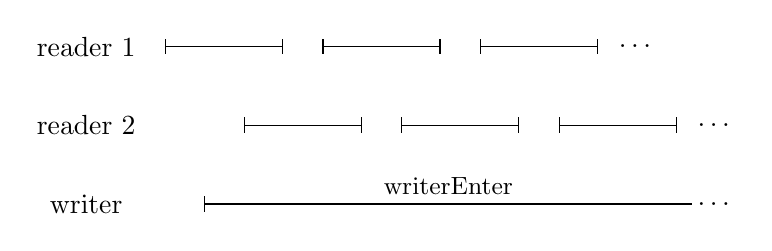
\begin{tikzpicture}
\draw (0,0) node{reader 1};
\draw[|-|] (1,0) -- (2.5,0); \draw[|-|] (3.0,0) -- (4.5,0); 
\draw[|-|] (5.0,0) -- (6.5,0); \draw (7.0,0) node{\ldots};
\draw (0,-1) node{reader 2}; 
\draw[|-|] (2.0,-1) -- (3.5,-1); \draw[|-|] (4.0,-1) -- (5.5,-1); 
\draw[|-|] (6.0,-1) -- (7.5,-1); \draw (8.0,-1) node{\ldots};
\draw (0,-2) node{writer}; 
\draw[|-] (1.5,-2) -- node[above]{\small\scalashape writerEnter} (7.7,-2);
\draw (8.0,-2) node{\ldots};
\end{tikzpicture}
\end{center}
%
The writer is starved: each time it receives a signal, if finds $\sm{readers}
> 0$, so has to wait again. 

Our second implementation avoids this problem.  The idea is that once a writer
calls |writerEnter|, no further reader will enter the critical region until a
writer enters and leaves.  Under the reasonable assumption that each current
reader eventually leaves, this will eventually allow a writer to enter.

The implementation is in Figures~\ref{fig:readers-writers-monitor-1} and
\ref{fig:readers-writers-monitor-2}. It maintains variables counting the
number of readers and writers currently waiting, so that exiting threads know
where to direct signals.  It uses two |Condition|s, for signalling to readers
or a writer that they can now enter.

%%%%%

\begin{figure}
\begin{scala}
class MonitorReadersWriters extends ReadersWritersLock{
  private var readers = 0
  private var writers = 0

  /** Number of readers waiting to enter. */
  private var readersWaiting = 0

  /** Number of writers waiting to enter. */
  private var writersWaiting = 0

  private val lock = new Lock

  /** Condition to signal to a waiting reader that it can now enter. */
  private val readerEnterC = lock.newCondition

  /** Condition to signal to a waiting writer that it can now enter. */
  private val writerEnterC = lock.newCondition

  ... // Continued in Figure £\sl\ref{fig:readers-writers-monitor-2}.£
}
\end{scala}
\caption{Improved implementation of a readers and writers lock (part~1).}
\label{fig:readers-writers-monitor-1}
\end{figure}

%%%%%

In each entry operation, if the thread has to wait it records that fact.  When
a reader exits, if it is the last reader to do so, and there is a writer
waiting, it signals to such a writer.  If this isn't the case, there is no
need to signal to a reader, because there can be no waiting reader at this
point: a reader waits only when $\sm{writers} > 0$ or $\sm{writersWaiting} >
0$, neither of which can be true.  When a writer exits, it prioritises
signalling to the waiting readers; but if there are none, it signals to a
waiting writer if there is one.

%%%%%

\begin{figure}
\begin{scala}
  def readerEnter() = lock.mutex{
    if(writers > 0 || writersWaiting > 0){ // Reader has to wait.
      readersWaiting += 1
      readerEnterC.await(writers == 0)
      readersWaiting -= 1
    }
    readers += 1
  }

  def readerExit() = lock.mutex{
    readers -= 1; assert(writers == 0)
    if(readers == 0 && writersWaiting > 0) writerEnterC.signal()
  }

  def writerEnter() = lock.mutex{
    if(readers > 0 || writers > 0){ // Writer has to wait.
      writersWaiting += 1
      writerEnterC.await(readers == 0 && writers == 0)
      writersWaiting -= 1
    }
    writers += 1
  }

  def writerExit() = lock.mutex{
    writers -= 1; assert(writers == 0 && readers == 0)
    if(readersWaiting > 0) readerEnterC.signalAll()
    else if(writersWaiting > 0) writerEnterC.signal()
  }

\end{scala}
\caption{Improved implementation of a readers and writers lock (part~2).}
\label{fig:readers-writers-monitor-2}
\end{figure}

%%%%%

This implementation is fair to writers.  Suppose there are one or more writers
waiting, but readers are currently in the critical region.  Then no more
readers will enter, and, by our earlier assumption, each of the current
readers will eventually leave.  The last such reader will signal to allow a
writer to enter.  This process will continue, so more writers will
subsequently enter.  In fact, the implementation of SCL |Condition|s is fair:
waiting threads will receive signals in the same order as they started
waiting.  This means that \emph{each} waiting writer will eventually enter the
critical region.  

The implementation is not quite fair to readers.  It is possible that when a
writer exits the critical region and signals to waiting readers, another
writer obtains the lock first, and so enters the critical region, preempting
the readers; the readers will wait again.  This process could repeat, so that
readers are starved.  However, this requires particularly unfortunate timing,
so seems unlikely.
